% ─────────────────────────────────────────────────────────────────────────────
% Análisis y rediseño del sistema de excepciones de OpenMarkov
% Compilar con: xelatex exception-report.tex
%   (requiere generar los PNG del diagrama PlantUML antes de compilar LaTeX;
%    véase el apartado "Generación de diagramas" en la introducción)
% ─────────────────────────────────────────────────────────────────────────────

\documentclass[11pt,a4paper]{article}

\usepackage[utf8]{inputenc}
\usepackage[T1]{fontenc}
\usepackage{lmodern}
\usepackage[spanish,es-tabla]{babel}
\usepackage[left=2.5cm,right=2.5cm,top=2.5cm,bottom=2.5cm]{geometry}
\usepackage{hyperref}
\usepackage{graphicx}
\usepackage{listings}
\usepackage{xcolor}
\usepackage{booktabs}
\usepackage{longtable}
\usepackage{array}
\usepackage{enumitem}
\usepackage{tcolorbox}
\usepackage{mdframed}
\usepackage{microtype}
\usepackage{parskip}
\usepackage{titlesec}
\usepackage{fancyhdr}
\usepackage{footnote}
\usepackage{tabularx}
\usepackage{multirow}
\usepackage{amssymb}

% Permite a TeX estirar espacios hasta 3em antes de declarar overfull hbox.
% Evita que nombres largos de clase Java se salgan del margen.
\emergencystretch=3em

% \jdot inserta un punto con punto de ruptura opcional tras él.
% Úsalo en nombres de clase con puntos: \texttt{WriterException\jdot NonProjectable...}
\newcommand{\jdot}{.\discretionary{}{}{}}

% ── Colores ──────────────────────────────────────────────────────────────────
\definecolor{codebackground}{RGB}{248,248,248}
\definecolor{codeborder}{RGB}{200,200,200}
\definecolor{keywordcolor}{RGB}{0,0,180}
\definecolor{commentcolor}{RGB}{100,150,100}
\definecolor{stringcolor}{RGB}{180,60,40}
\definecolor{problemred}{RGB}{220,50,50}
\definecolor{okgreen}{RGB}{30,140,60}
\definecolor{warnOrange}{RGB}{200,100,0}
\definecolor{newblue}{RGB}{30,80,180}
\definecolor{lightred}{RGB}{255,230,230}
\definecolor{lightgreen}{RGB}{230,255,235}
\definecolor{lightblue}{RGB}{230,240,255}
\definecolor{lightyellow}{RGB}{255,252,220}

% ── Listados de código ────────────────────────────────────────────────────────
\lstset{
    basicstyle=\ttfamily\small,
    backgroundcolor=\color{codebackground},
    frame=single,
    rulecolor=\color{codeborder},
    breaklines=true,
    breakatwhitespace=true,
    tabsize=4,
    showstringspaces=false,
    keywordstyle=\color{keywordcolor}\bfseries,
    commentstyle=\color{commentcolor}\itshape,
    stringstyle=\color{stringcolor},
    language=Java,
    xleftmargin=6pt,
    xrightmargin=6pt,
    aboveskip=8pt,
    belowskip=6pt,
    captionpos=b,
    numbers=left,
    numberstyle=\tiny\color{gray},
    numbersep=8pt,
    morekeywords={record,sealed,permits,var},
}

% ── Cajas de advertencia / propuesta ─────────────────────────────────────────
\tcbuselibrary{skins,breakable}

\newtcolorbox{problemabox}[1][]{
    colback=lightred,
    colframe=problemred,
    fonttitle=\bfseries\small,
    title={\color{problemred}\textbf{Problema:} #1},
    breakable,
    left=6pt, right=6pt, top=4pt, bottom=4pt,
}

\newtcolorbox{propuestabox}[1][]{
    colback=lightblue,
    colframe=newblue,
    fonttitle=\bfseries\small,
    title={\color{newblue}\textbf{Propuesta:} #1},
    breakable,
    left=6pt, right=6pt, top=4pt, bottom=4pt,
}

\newtcolorbox{consecuenciabox}[1][]{
    colback=lightyellow,
    colframe=warnOrange,
    fonttitle=\bfseries\small,
    title={\color{warnOrange}\textbf{Consecuencia:} #1},
    breakable,
    left=6pt, right=6pt, top=4pt, bottom=4pt,
}

\newtcolorbox{nuevabox}[1][]{
    colback=lightgreen,
    colframe=okgreen,
    fonttitle=\bfseries\small,
    title={\color{okgreen}\textbf{Añadido en esta revisión:} #1},
    breakable,
    left=6pt, right=6pt, top=4pt, bottom=4pt,
}

% ── Cabeceras ─────────────────────────────────────────────────────────────────
\pagestyle{fancy}
\fancyhf{}
\fancyhead[L]{\small\textit{OpenMarkov — Sistema de excepciones}}
\fancyhead[R]{\small\textit{Marzo 2026}}
\fancyfoot[C]{\thepage}
\renewcommand{\headrulewidth}{0.4pt}

% ── Secciones ─────────────────────────────────────────────────────────────────
\titleformat{\section}{\large\bfseries}{}{0em}{\thesection\quad}[\titlerule]
\titleformat{\subsection}{\normalsize\bfseries}{}{0em}{\thesubsection\quad}
\titleformat{\subsubsection}{\normalsize\itshape\bfseries}{}{0em}{\thesubsubsection\quad}

% ── Metadatos del documento ───────────────────────────────────────────────────
\hypersetup{
    pdfauthor={OpenMarkov — Análisis de código},
    pdftitle={Análisis y rediseño del sistema de excepciones de OpenMarkov},
    colorlinks=true,
    linkcolor=newblue,
    urlcolor=newblue,
}

% ─────────────────────────────────────────────────────────────────────────────
\begin{document}

\begin{titlepage}
    \centering
    \vspace*{2cm}
    {\Large\bfseries Análisis y rediseño del sistema de excepciones\par}
    \vspace{0.5em}
    {\large\bfseries OpenMarkov 0.3.0-SNAPSHOT\par}
    \vspace{1.5em}
    {\normalsize Informe técnico — Marzo 2026\par}
    \vspace{1em}
    \rule{0.6\textwidth}{0.4pt}\par
    \vspace{1em}
    {\small
        Inventario completo de las excepciones del proyecto,\par
        análisis detallado de los problemas identificados y sus consecuencias,\par
        diagramas UML de la jerarquía actual y de la jerarquía rediseñada,\par
        y plan de migración por fases.\par
    }
    \vspace{1.5em}
    \textbf{Nota sobre los diagramas PlantUML}\par
    \vspace{0.4em}
    {\small
        Los diagramas de este documento se generan con PlantUML a partir de los ficheros\\
        \texttt{exception-hierarchy-current.puml} y \texttt{exception-hierarchy-proposed.puml}.\\
        Para regenerarlos: \texttt{java -jar plantuml.jar *.puml -tpng}\\
        O con \texttt{plantumlc} si está disponible en el PATH.
    }
    \vfill
    {\small CISIAD — Universidad Nacional de Educación a Distancia (UNED)\par}
\end{titlepage}

\tableofcontents
\newpage

% ─────────────────────────────────────────────────────────────────────────────
\section{Qué es una excepción y por qué su diseño importa}
% ─────────────────────────────────────────────────────────────────────────────

En cualquier programa Java, una \textbf{excepción} es el mecanismo formal mediante el cual una
pieza de código avisa a sus llamadores de que algo ha salido mal y de que no puede continuar
normalmente. Cuando ocurre un problema, el código \guillemotleft lanza\guillemotright  (en inglés, \textit{throws}) una
excepción; el código que llamó al primero tiene entonces la oportunidad de \guillemotleft capturarla\guillemotright 
(en inglés, \textit{catch}) y tomar alguna medida correctiva, o bien dejar que siga
propagándose hacia capas más externas del programa.

El lenguaje Java establece una distinción fundamental entre dos tipos de excepciones:

\begin{description}[leftmargin=2em]
    \item[\textbf{Excepciones comprobadas} (\textit{checked})]
        Son aquellas que Java obliga a declarar explícitamente en la firma de cada método que
        puede lanzarlas. Cualquier método que llame a otro que declare una excepción comprobada
        tiene dos únicas opciones legales: capturarla allí mismo, o declarar a su vez que él
        también puede lanzarla. Esto crea una \emph{cadena de responsabilidad formal} a lo largo
        de toda la pila de llamadas. El objetivo original de este mecanismo es obligar al
        programador a pensar en los errores recuperables: aquellos ante los cuales el llamador
        puede hacer algo útil (mostrar un mensaje al usuario, intentar una alternativa, etc.).

    \item[\textbf{Excepciones no comprobadas} (\textit{unchecked})]
        Son aquellas que representan errores de programación o estados internamente imposibles:
        un puntero nulo, un índice fuera de rango, una suposición de diseño que se ha violado.
        Java \emph{no} obliga a declararlas ni a capturarlas. Se propagan automáticamente hasta
        que alguien las atrapa (normalmente en la capa más externa del programa, que las muestra
        como un error interno) o hasta que terminan el programa con un volcado de pila de llamadas.
\end{description}

El diseño adecuado del sistema de excepciones de una aplicación es un \textbf{contrato de
comunicación entre capas}: indica claramente qué puede fallar de forma recuperable, qué representa
un error de programación y qué simplemente no puede ocurrir en condiciones normales. Un sistema
de excepciones mal diseñado deteriora ese contrato, hace que los errores sean invisibles o
difíciles de diagnosticar, y aumenta significativamente el coste de mantenimiento.

% ─────────────────────────────────────────────────────────────────────────────
\section{Estado actual del sistema}
% ─────────────────────────────────────────────────────────────────────────────

\subsection{Inventario}

El proyecto define \textbf{62 clases de excepción propias}, distribuidas entre seis módulos. Casi
todas son comprobadas (\textit{checked}), salvo dos (\texttt{UnreacheableException} y
\texttt{UnrecoverableException}, que son \textit{unchecked}).

\begin{longtable}{llr}
    \toprule
    \textbf{Módulo} & \textbf{Paquete principal} & \textbf{Clases} \\
    \midrule
    \texttt{core}                       & \texttt{org.openmarkov.core.exception}        & 27 \\
    \texttt{gui}                        & \texttt{org.openmarkov.gui.exception}          & 27 \\
    \texttt{io}                         & \texttt{org.openmarkov.io.probmodel.exception} &  1 \\
    \texttt{learning.core}              & \texttt{org.openmarkov.learning.core.exception}&  2 \\
    \texttt{learning.gui}               & \texttt{org.openmarkov.learning.exception}     &  2 \\
    \texttt{stochasticPropagationOutput}& (módulo propio)                               &  1 \\
    \midrule
    \textbf{Total}                      &                                               & \textbf{62} \\
    \bottomrule
\end{longtable}

\subsection{Patrón de clases internas}

Doce excepciones actúan como \emph{namespaces} de variantes, agrupando múltiples situaciones
de error bajo una excepción base común mediante clases internas estáticas:

\begin{longtable}{lr}
    \toprule
    \textbf{Excepción base} & \textbf{Variantes internas} \\
    \midrule
    \texttt{ConstraintViolatedException}  & 42 \\
    \texttt{ParserException}              & 15 \\
    \texttt{PGMXParserException}          & 14 \\
    \texttt{NonProjectablePotentialException} & 8 \\
    \texttt{WriterException}              & 6  \\
    \texttt{DoEditException}              & 5  \\
    \texttt{CostEffectivenessException}   & 4  \\
    \texttt{IncompatibleEvidenceException}& 3  \\
    \texttt{NotEvaluableNetworkException} & 3  \\
    \texttt{InvalidNetworkTypeException}  & 2  \\
    \texttt{LearningException}            & 2  \\
    \texttt{PotentialOperationException}  & 1  \\
    \bottomrule
\end{longtable}

\subsection{Interfaces de localización}

Existe un sistema dual de interfaces:

\begin{itemize}
    \item \texttt{IOpenMarkovException} — interfaz base para todas las excepciones propias;
          incluye métodos para obtener el mensaje y el título de la excepción.
    \item \texttt{IBundledOpenMarkovException} — extiende la anterior; añade soporte para
          mensajes localizados en ficheros \texttt{.properties}, de forma que los diálogos de
          error puedan mostrarse en el idioma del usuario.
\end{itemize}

No todas las excepciones implementan estas interfaces de forma consistente.

\subsection{Diagrama de la jerarquía actual}

Las figuras~\ref{fig:jerarquia-actual-a} y~\ref{fig:jerarquia-actual-b} muestran la jerarquía
de excepciones tal como está implementada en la versión 0.3.0-SNAPSHOT. Las excepciones
sombreadas en \textcolor{problemred}{rojo} son aquellas que el propio código fuente identifica,
mediante comentarios \texttt{TODO}, como candidatas a convertirse en \textit{unchecked}.
Las sombreadas en \textcolor{warnOrange}{naranja} no habían sido analizadas en ningún informe
previo sobre el sistema de excepciones.

\begin{figure}[htbp]
    \centering
    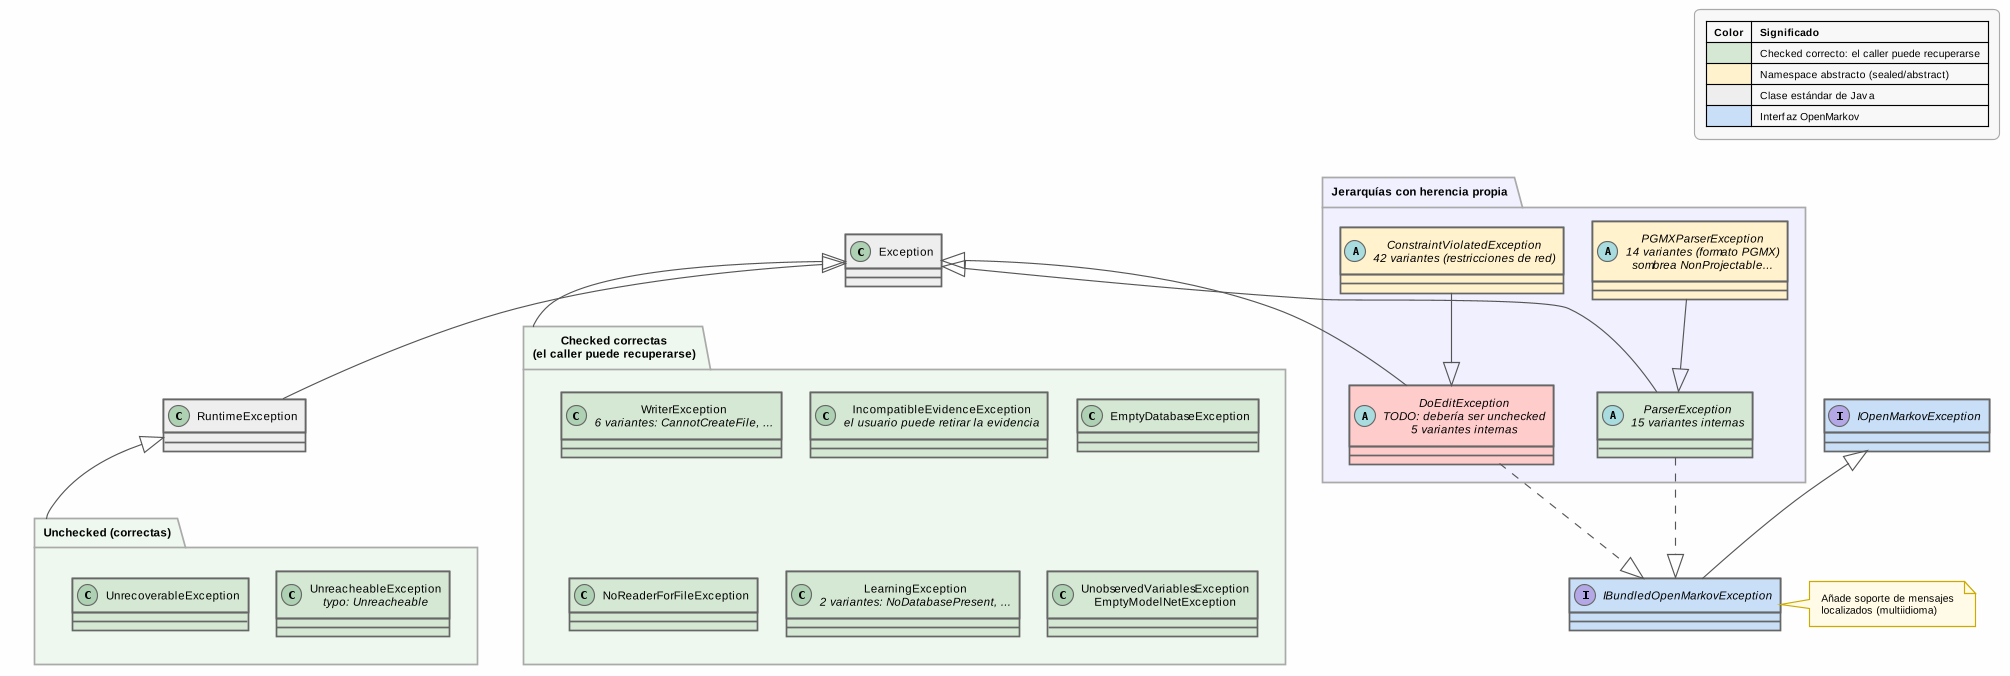
\includegraphics[width=\textwidth,keepaspectratio]{exception-hierarchy-current-a}
    \caption{Jerarquía de excepciones actual (parte~1): excepciones correctamente diseñadas
             y jerarquías con herencia propia. Fuente: \texttt{exception-hierarchy-current-a.puml}.}
    \label{fig:jerarquia-actual-a}
\end{figure}

\begin{figure}[htbp]
    \centering
    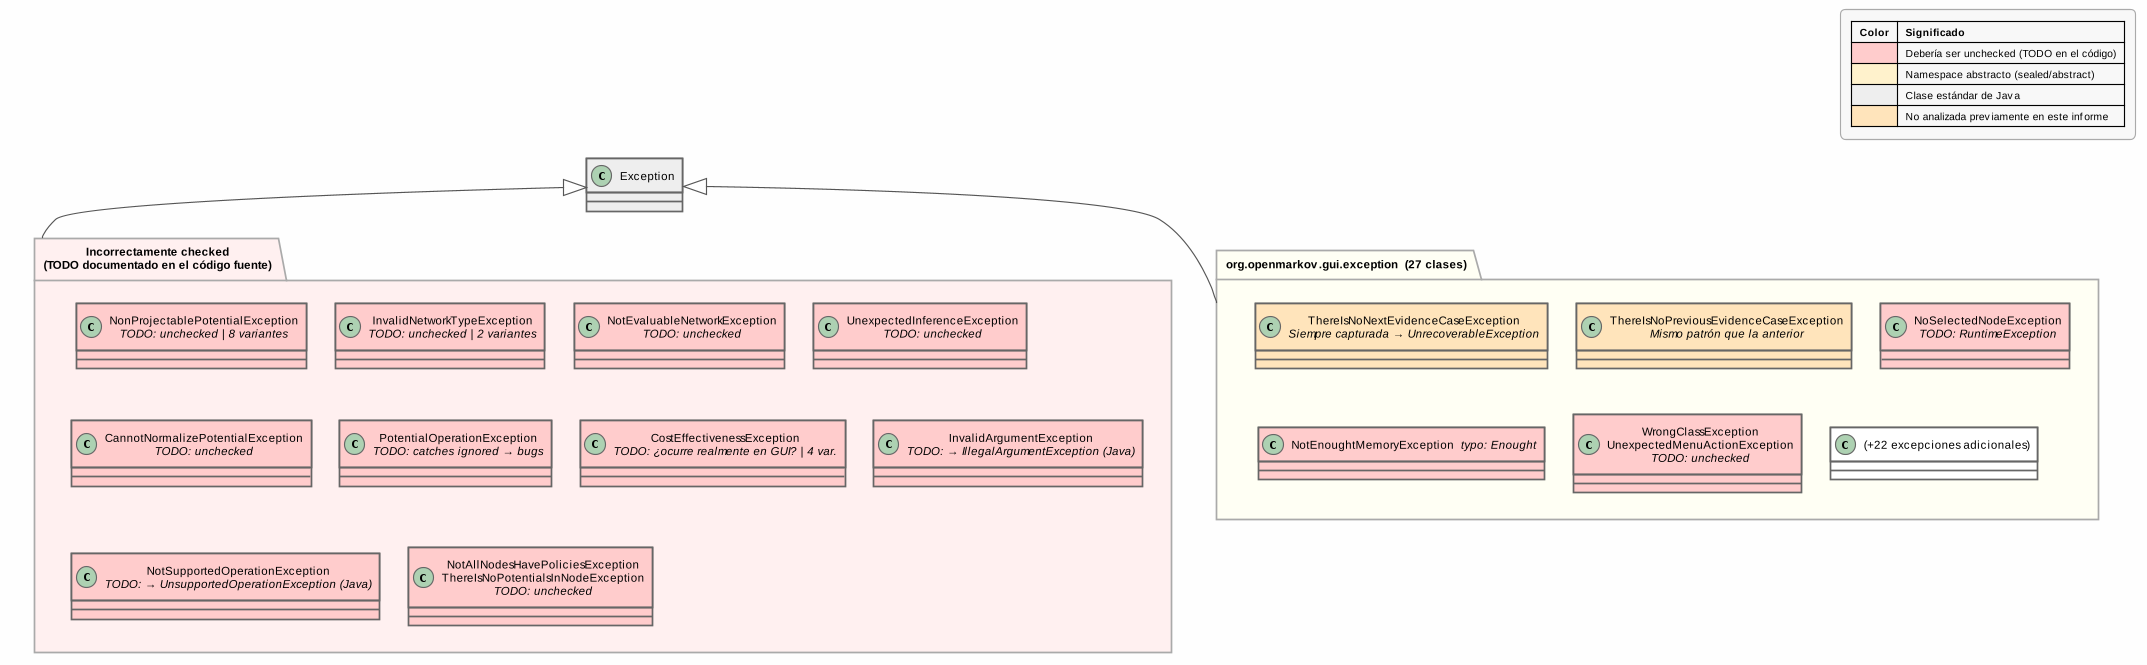
\includegraphics[width=\textwidth,keepaspectratio]{exception-hierarchy-current-b}
    \caption{Jerarquía de excepciones actual (parte~2): excepciones incorrectamente
             declaradas como \textit{checked} y excepciones del módulo GUI.
             Fuente: \texttt{exception-hierarchy-current-b.puml}.}
    \label{fig:jerarquia-actual-b}
\end{figure}

\newpage

% ─────────────────────────────────────────────────────────────────────────────
\section{Problemas identificados}
% ─────────────────────────────────────────────────────────────────────────────

\subsection{El exceso de excepciones comprobadas que nadie puede resolver}

\subsubsection{Descripción del problema}

En Java, declarar una excepción como \textit{checked} es una promesa al llamador: \guillemotleft Si me
llamas, es posible que ocurra este error, y \emph{tienes} alguna forma de manejarlo.\guillemotright 
El mecanismo tiene sentido cuando el llamador dispone de una alternativa real: si no se puede
abrir un fichero, puede pedir al usuario que indique otro; si la red no tiene nodos, puede
mostrar un aviso y detener la operación con elegancia.

Sin embargo, OpenMarkov declara como comprobadas \textbf{19 excepciones ante las cuales ningún
llamador puede hacer nada útil}. El propio código fuente lo reconoce explícitamente: cada uno
de esos 19 ficheros contiene un comentario \texttt{TODO} admitiendo que la excepción debería
ser \textit{unchecked}. Los siguientes son extractos literales de esos comentarios:

\begin{itemize}[nosep]
    \item \texttt{DoEditException}: \textit{\guillemotleft Either design is poor, or the exceptions it encloses
          could be turned into RuntimeExceptions.\guillemotright }
    \item \texttt{NonProjectablePotentialException}: \textit{\guillemotleft Almost every exception of this class
          is wrapped into an \texttt{UnreacheableException} or shown with \texttt{JOptionPane}.
          This might be a RuntimeException.\guillemotright }
    \item \texttt{NotSupportedOperationException}: \textit{\guillemotleft Exceptions of this type are always
          caught and then ignored. Perhaps they should be turned into RuntimeExceptions.\guillemotright }
\end{itemize}

\subsubsection{Qué ocurre en la práctica}

Cuando un programador llama a un método que declara una excepción \textit{checked} que sabe que
no puede manejar, tiene dos opciones, ninguna de ellas buena:

\begin{enumerate}
    \item \textbf{Capturarla y no hacer nada}: el código atrapa la excepción, ignora el error, y
          el programa continúa en un estado posiblemente inconsistente. El usuario no ve ningún
          aviso; el desarrollador no recibe ninguna traza. Este patrón, conocido como
          \emph{excepción tragada} (\textit{swallowed exception}), es una de las principales
          causas de errores silenciosos difíciles de reproducir.

    \item \textbf{Envolverla en una excepción \textit{unchecked} y relanzarla}: el código atrapa
          la excepción, la mete dentro de una \textit{unchecked} (en OpenMarkov,
          \texttt{UnreacheableException} o \texttt{UnrecoverableException}), y la lanza de nuevo.
          El resultado final es idéntico a haber declarado la excepción como \textit{unchecked}
          desde el principio, pero con el coste de haber obligado a \emph{todos} los métodos
          intermedios de la pila de llamadas a declarar o capturar la excepción original.
\end{enumerate}

\begin{consecuenciabox}[Propagación burocrática en cascada]
    En OpenMarkov, el método \texttt{MainPanelListenerAssistant.actionPerformed()} —el punto
    central de control de la interfaz gráfica— captura un bloque de \textbf{siete excepciones
    distintas} más de veinte veces a lo largo de sus 380 líneas, relanzándolas todas como
    \texttt{UnrecoverableException}. Ese bloque se repite prácticamente idéntico en cada
    acción. La causa directa es que los métodos invocados declaran excepciones comprobadas que
    la GUI no puede resolver; el resultado es 200+ líneas de código de gestión de errores que
    no gestiona nada, solo propaga.
\end{consecuenciabox}

\subsubsection{Las 19 excepciones candidatas a \textit{unchecked}}

{\small
\begin{longtable}{p{7.5cm}p{7.5cm}}
    \toprule
    \textbf{Excepción} & \textbf{Argumento del TODO en el código} \\
    \midrule
    \texttt{DoEditException}                    & El diseño es deficiente o las excepciones que encapsula podrían ser \textit{unchecked} \\
    \texttt{IncompatibleEvidenceException}       & Capturada e ignorada en casi todos los bloques catch, lo que probablemente genera bugs inesperados \\
    \texttt{NonProjectable\-Potential\-Exception}   & Casi siempre envuelta en \texttt{UnreacheableException} o mostrada con \texttt{JOptionPane} \\
    \texttt{NotEvaluableNetworkException}        & Solo se captura para mostrar un mensaje genérico \\
    \texttt{NotSupportedOperationException}      & Siempre capturada y luego ignorada \\
    \texttt{InvalidArgumentException}            & Podría ser una \textit{RuntimeException} \\
    \texttt{UnexpectedInferenceException}        & Las capturas siempre la envuelven con \texttt{UnreacheableException} \\
    \texttt{InvalidNetworkTypeException}         & Siempre envuelta en \texttt{UnreacheableException} \\
    \texttt{CannotNormalizePotentialException}   & ¿Realmente ocurre en la GUI? \\
    \texttt{CostEffectivenessException}          & ¿Realmente ocurre en la GUI? \\
    \texttt{NotAllNodesHavePoliciesException}    & Capturada y lanzada como \texttt{UnreacheableException} \\
    \texttt{PotentialOperationException}         & Las capturas solo la muestran y la ignoran, generando bugs posteriores \\
    \texttt{WrongClassException}                 & Probablemente debería ser \texttt{UnreacheableException} \\
    \texttt{UnexpectedMenuActionException}       & Probablemente debería ser \texttt{UnreacheableException} \\
    \texttt{NoSelectedNodeException}             & Probablemente debería ser \textit{RuntimeException} \\
    \texttt{IntervalsAreNotEvenException}        & ¿Realmente ocurre en la GUI? \\
    \texttt{IntervalsAreNotMultipleOf3Exception} & ¿Realmente ocurre en la GUI? \\
    \texttt{NonProjectable\-Potential\-Exception\jdot Can\-not\-Evaluate} & Solo se usa una vez y se envuelve en \texttt{UnreacheableException} \\
    \texttt{ThereIsNoPotentials\-InNodeException} & Capturada y relanzada como \textit{unchecked} \\
    \bottomrule
\end{longtable}
}

\subsection{La firma genérica \texttt{throws Exception}}

\subsubsection{Descripción del problema}

Java permite declarar \texttt{throws Exception} en la firma de un método, lo que significa
\guillemotleft este método puede lanzar cualquier excepción posible\guillemotright . Es el equivalente en el lenguaje de
firmar un contrato en blanco: el llamador no sabe qué puede fallar ni bajo qué condiciones.

OpenMarkov tiene \textbf{82 firmas de método} que declaran \texttt{throws Exception} sin
especificar tipo. La mayoría se concentran en el ciclo de aprendizaje automático
(\texttt{LearningAlgorithm\jdot getBestEdit()}, \texttt{LearningAlgorithm\jdot getNextEdit()}) y en
los \textit{callbacks} de plugins.

\begin{consecuenciabox}[Contratos de API opacos]
    Cuando un método declara \texttt{throws Exception}, el llamador se ve forzado a capturar
    \texttt{Exception} (la clase más genérica posible) o a declarar a su vez \texttt{throws
    Exception}, propagando el problema. Ningún compilador ni herramienta de análisis estático
    puede indicar al desarrollador qué situaciones de error debe contemplar realmente. En la
    práctica, los desarrolladores suelen capturar \texttt{Exception} con un bloque vacío o con
    un log genérico, perdiendo toda información sobre la causa real del fallo.
\end{consecuenciabox}

\subsection{El silenciamiento silencioso: \texttt{catch → return null}}

\subsubsection{Descripción del problema}

En el fichero \texttt{FormatManager.java} (líneas 63--78) existe un bloque que carga dinámicamente
los plugins de lectura de formatos de archivo. Cuando un plugin no se puede instanciar correctamente
(por ejemplo, porque le falta una clase en el classpath, o porque su constructor lanza una excepción),
el código captura el error y devuelve \texttt{null}, sin registrar ningún mensaje en el log y sin
avisar al sistema de que el plugin ha fallado:

\begin{lstlisting}[caption={Antipatrón en \texttt{FormatManager.java} — error silenciado},label={lst:formatmanager}]
// FormatManager.java, líneas 63-78
.map(readerClass -> {
    try {
        return readerClass.getDeclaredConstructor().newInstance();
    } catch (InstantiationException | NoSuchMethodException
           | IllegalAccessException | InvocationTargetException e) {
        return null;  // <-- error silenciado; el reader queda null
    }
})
\end{lstlisting}

\subsubsection{Por qué es peligroso}

Este patrón —conocido como \textit{excepción tragada con retorno nulo} (\textit{catch-and-return-null})—
introduce una \textbf{bomba de relojería} en el sistema. En el momento en que ocurre el error, el
código no hace nada observable; la lista de plugins simplemente contiene un elemento \texttt{null}
donde debería haber un lector funcional.

El fallo real no se manifiesta en ese punto sino \emph{más adelante}, cuando algún otro código
intenta usar ese \texttt{null} como si fuera un lector válido. En ese momento se produce una
\texttt{NullPointerException} que no tiene ninguna relación visible con la causa original: el
desarrollador verá un error en un lugar completamente distinto de aquel donde ocurrió el
problema real, con una traza que no contiene ninguna referencia al plugin que falló ni al motivo
por el que falló.

\begin{consecuenciabox}[Diagnóstico imposible]
    Si un usuario instala un plugin de formato de archivo mal empaquetado, OpenMarkov no le
    mostrará ningún aviso. El sistema simplemente ignorará ese formato. El usuario solo
    descubrirá el problema cuando intente abrir o guardar un fichero de ese tipo, y en ese
    momento el mensaje de error no le indicará que el plugin es el responsable.
\end{consecuenciabox}

\subsection{Conflictos de nombres entre clases internas}

\subsubsection{Descripción del problema}

Dos clases internas tienen el mismo nombre que otras excepciones ya existentes en el proyecto:

\begin{itemize}
    \item \texttt{WriterException\jdot NonProjectablePotentialException} tiene el mismo nombre que
          \texttt{org\jdot openmarkov\jdot core\jdot exception\jdot NonProjectablePotentialException}.
    \item \texttt{PGMXParserException\jdot EvidenceIsIncompatibleWithOther} tiene el mismo nombre que
          \texttt{IncompatibleEvidenceException\jdot EvidenceIsIncompatibleWithOther}.
\end{itemize}

\subsubsection{Por qué es peligroso}

En Java, cuando se usa el nombre corto de una clase (sin el paquete completo) dentro de un
fichero que tiene acceso a dos clases con ese mismo nombre, el compilador resuelve la ambigüedad
usando la que está \emph{más cerca} en el ámbito. Esto se denomina \textit{sombreado de nombres}
(\textit{name shadowing}). El resultado práctico es que un desarrollador que escribe código en
los módulos afectados puede estar usando \emph{sin saberlo} la clase interna en lugar de la clase
raíz, o viceversa.

En ambos casos citados, la clase interna y la clase raíz representan el mismo concepto de error,
lo que confirma que se trata de código duplicado. Si en el futuro se modifica el comportamiento
de la clase raíz (por ejemplo, añadiendo un nuevo campo de información de diagnóstico), la clase
interna no recibirá esa mejora automáticamente, y el sistema presentará comportamientos
inconsistentes dependiendo de qué excepción se lance en cada punto del código.

\subsection{Errores ortográficos en nombres de clase}

\subsubsection{Descripción del problema}

Ocho clases de excepción tienen errores tipográficos en su nombre. Los nombres de las clases
en Java son parte de la API pública y, en el caso de las excepciones, aparecen directamente en
los mensajes de error y en las trazas de pila que ven los desarrolladores.

{\small
\begin{longtable}{p{8cm}p{7cm}}
    \toprule
    \textbf{Nombre actual (incorrecto)} & \textbf{Nombre correcto} \\
    \midrule
    \texttt{UnsatisfiedContraints}                & \texttt{UnsatisfiedConstraints} \\
    \texttt{SamplesWeigthIsZero}                  & \texttt{SamplesWeightIsZero} \\
    \texttt{MissingPropertiesOfContiousVariable}  & \texttt{MissingProperties\-OfContinuousVariable} \\
    \texttt{CannotAsignPotentialToStaticVariable} & \texttt{CannotAssignPotential\-ToStaticVariable} \\
    \texttt{TriedToSplitInverval\-OutsideBoundsException} & \texttt{TriedToSplitInterval\-OutsideBoundsException} \\
    \texttt{ValueOutOfDomaingRangeException}      & \texttt{ValueOutOfDomainRangeException} \\
    \texttt{NotEnoughtMemoryException}            & \texttt{NotEnoughMemoryException} \\
    \texttt{UnreacheableException}                & \texttt{UnreachableException} \\
    \bottomrule
\end{longtable}
}

\subsubsection{Por qué importa}

Los nombres incorrectos de clase aparecen en: las trazas de pila de error que ven los
desarrolladores, los registros de log, la documentación generada automáticamente (Javadoc), y
los resultados de búsquedas en el código. Un desarrollador que busque \texttt{unreachable} no
encontrará \texttt{UnreacheableException}. Un desarrollador que busque \texttt{constraint} no
encontrará \texttt{UnsatisfiedContraints}. Los nombres con errores ortográficos actúan como
\emph{ruido} en el sistema de búsqueda e indexación del código.

\subsection{Detalles técnicos internos expuestos en las APIs públicas}

\subsubsection{Descripción del problema}

Varios métodos públicos de los módulos de I/O declaran explícitamente excepciones de las
bibliotecas que usan internamente:

\begin{lstlisting}[caption={API que expone detalles de implementación},label={lst:api-exposicion}]
// Antes — API acoplada a la tecnología de implementación
public ProbNetReader getProbNetReader(URL url)
    throws SAXException, IOException,
           NoReaderForFileException, ParserException;
\end{lstlisting}

\texttt{SAXException} es una excepción específica de la biblioteca SAX, que es la biblioteca de
análisis de XML elegida internamente. \texttt{IOException} es una excepción de Java para
operaciones de entrada/salida de bajo nivel.

\subsubsection{Por qué es peligroso}

Un llamador de este método —por ejemplo, la interfaz gráfica— tiene que importar y conocer
\texttt{SAXException} aunque nunca haya decidido usar SAX para nada. Si en el futuro se decide
cambiar la implementación del parser XML (por ejemplo, de SAX a StAX o a JDOM), \emph{todos los
llamadores del método} tendrán que actualizarse, aunque para ellos el cambio sea completamente
transparente: su trabajo es \guillemotleft abrir una red\guillemotright , no \guillemotleft analizar XML con SAX\guillemotright . Este acoplamiento
innecesario entre capas hace que cambios internos de implementación tengan un impacto externo
mucho mayor del que deberían tener.

La regla general es que una API pública solo debe exponer excepciones definidas en términos del
\emph{dominio del problema}, no de los detalles de su implementación.

\subsection{Excepciones \textit{checked} que cruzan capas incorrectas}

\subsubsection{Descripción del problema}

\texttt{DoEditException} está definida en el módulo \texttt{core} —la capa de dominio más
baja— y aparece en \textbf{113 firmas de método} distribuidas por todos los módulos del
proyecto: \texttt{gui}, \texttt{learning.algorithm}, \texttt{learning.gui}, etc.

\subsubsection{Qué significa cruzar capas incorrectas}

En una arquitectura bien estructurada, las dependencias entre capas fluyen en una sola
dirección: desde las capas externas (GUI, aprendizaje) hacia las capas internas (dominio,
modelo). Una excepción definida en la capa interna puede ser usada por las capas externas, pero
no debería \emph{obligar} a esas capas a declarar y gestionar detalles de la capa interna.

Cuando \texttt{DoEditException} —una excepción de la capa de dominio más básica— aparece en
firmas de la GUI, obliga a la interfaz gráfica a conocer y gestionar el vocabulario de errores
del motor de edición. Cualquier programador que trabaje en la GUI debe entender qué es un
\textit{edit} de dominio para poder manejar correctamente el error. Esto viola el principio de
separación de responsabilidades: la GUI debería poder gestionar errores de UI sin necesidad de
conocer los mecanismos internos del modelo de dominio.

\begin{consecuenciabox}[Acoplamiento excesivo entre capas]
    En la práctica, los 113 métodos que declaran \texttt{DoEditException} en capas superiores
    no hacen nada útil con ella: simplemente la relanzán como \texttt{UnrecoverableException}
    o la muestran con un \texttt{JOptionPane}. El único efecto real es que todos esos métodos
    \emph{tienen que importar} el paquete \texttt{org.openmarkov.core.exception}, creando
    dependencias de compilación innecesarias.
\end{consecuenciabox}

\subsection[Las excepciones de navegación de evidencia]{Las excepciones de navegación de evidencia:
\texttt{ThereIsNoNext\-Evidence\-Case\-Exception} y
\texttt{ThereIsNoPrevious\-Evidence\-Case\-Exception}}

\subsubsection{Descripción del problema}

\texttt{ThereIsNoNextEvidenceCaseException} y \texttt{ThereIsNoPreviousEvidenceCaseException}
son excepciones comprobadas del módulo \texttt{gui}. Se lanzan cuando el usuario intenta navegar
(con los botones \guillemotleft caso siguiente\guillemotright  o \guillemotleft caso anterior\guillemotright ) más allá del límite de la lista de casos
de evidencia.

Ambas tienen una implementación mínima —sin campos adicionales, sin información contextual— y
son siempre capturadas en \texttt{MainPanelListenerAssistant} para ser inmediatamente relanzadas
como \texttt{UnrecoverableException}:

\begin{lstlisting}[caption={Patrón real de uso de estas excepciones en la GUI},label={lst:evidence-nav}]
case GO_TO_NEXT_EVIDENCE_CASE -> {
    try {
        evidenceCasesNavigationOption("GO_TO_NEXT_EVIDENCE_CASE");
    } catch (NotEvaluableNetworkException
           | NonProjectablePotentialException
           | NotEnoughtMemoryException
           | IncompatibleEvidenceException
           | CannotNormalizePotentialException
           | ThereIsNoNextEvidenceCaseException      // <-- declarada
           | ThereIsNoPreviousEvidenceCaseException  // <-- declarada
           | ConstraintViolatedException ex) {
        throw new UnrecoverableException(ex);  // relanzada sin tratamiento
    }
}
\end{lstlisting}

Este mismo bloque de siete excepciones se repite \emph{seis veces} para los seis botones de
navegación (primero, anterior, siguiente, último, nuevo caso, borrar todo).

\subsubsection{Consecuencia}

Estas excepciones \emph{podrían} ser útiles: saber que el usuario ha llegado al final de la
lista de evidencias es información relevante que podría usarse para deshabilitar el botón
\guillemotleft siguiente\guillemotright  antes de que el usuario lo pulse. Sin embargo, en la implementación actual, ese
razonamiento no ocurre: la excepción se lanza \emph{después} del intento fallido, se captura,
y se relanza como error irrecuperable, lo que probablemente resulta en mostrar un mensaje de
error al usuario en lugar de simplemente deshabilitar el botón.

La corrección no es solo cambiar el tipo de la excepción, sino repensar la lógica: el límite
de la lista de evidencias debe consultarse \emph{antes} de intentar navegar, para que los
botones reflejen correctamente el estado.

\subsection{Pérdida del rastro del error al envolver \texttt{DoEditException}}

\subsubsection{Descripción del problema}

En \texttt{Node.java} (línea 807), cuando se captura una \texttt{NonProjectablePotentialException}
y se envuelve en una \texttt{DoEditException}, se comete el siguiente error:

\begin{lstlisting}[caption={Pérdida del rastro de la excepción original en \texttt{Node.java}},label={lst:node-stacktrace}]
// Node.java, línea ~807 — MAL
} catch (NonProjectablePotentialException e) {
    throw new DoEditException.CannotDoEditException(e.getMessage()); // ← solo el mensaje
}

// CORRECTO: pasar la excepción original como causa
} catch (NonProjectablePotentialException e) {
    throw new DoEditException.CannotDoEditException(e);  // ← causa completa
}
\end{lstlisting}

\subsubsection{Qué se pierde}

Cuando se lanza una nueva excepción pasando únicamente \texttt{e.getMessage()} en lugar de
\texttt{e} (la excepción completa), se pierde la \emph{causa raíz} (\textit{cause}). En términos
prácticos, esto significa que la traza de pila (\textit{stack trace}) que finalmente llega al
log de la aplicación o al desarrollador \textbf{no contiene ninguna información sobre dónde
se originó el error real}. Solo se ve el punto donde se lanzó la \texttt{DoEditException}, no
el punto donde falló el cálculo de probabilidades que la provocó.

Imagine que un operario de una planta química reporta: \guillemotleft Ha habido un problema.\guillemotright  Sin indicar
dónde, en qué equipo, ni bajo qué condiciones. El rastro es la diferencia entre un diagnóstico
en segundos y una búsqueda que puede durar horas.

\subsection{Re-lanzamiento vacío en \texttt{ProbNet.setNetworkType()}}

\subsubsection{Descripción del problema}

En \texttt{ProbNet.java} (líneas 362--368) existe el siguiente bloque:

\begin{lstlisting}[caption={Re-lanzamiento vacío en \texttt{ProbNet.setNetworkType()}},label={lst:relaunch-empty}]
// ProbNet.java, líneas 362-368
public void setNetworkType(NetworkType networkType)
        throws ConstraintViolatedException {
    try {
        // ... lógica de cambio de tipo
    } catch (ConstraintViolatedException e) {
        throw e;  // relanza sin ningún tratamiento adicional
    }
}
\end{lstlisting}

El bloque \texttt{try/catch} captura \texttt{ConstraintViolatedException} y la relanza
inmediatamente, sin agregar ningún mensaje, sin registrar ningún log, sin modificar la excepción
en modo alguno.

\subsubsection{Por qué es un problema}

Un bloque \texttt{try/catch} que no realiza ningún tratamiento es código muerto con un coste:
añade un nivel innecesario en la pila de llamadas (y por tanto en la traza de error), introduce
ruido visual en el código que dificulta entender el flujo real, y puede confundir a futuros
desarrolladores haciéndoles creer que hay algún tratamiento implícito que en realidad no existe.

La excepción podría declararse directamente en la firma del método y dejar que se propagase
sola, eliminando el \texttt{try/catch} sin ningún cambio de comportamiento.

\newpage

% ─────────────────────────────────────────────────────────────────────────────
\section{Propuestas de rediseño}
% ─────────────────────────────────────────────────────────────────────────────

\subsection{Propuesta A — Convertir a \textit{unchecked} las excepciones no recuperables}

\textbf{Impacto: alto. Riesgo: medio.}

Las 19 excepciones identificadas en el apartado 3.1 deben convertirse en \textit{RuntimeException}.
El criterio es preciso: si el llamador nunca puede hacer nada útil al capturar una excepción más
que mostrar un mensaje de error genérico o relanzarla, esa excepción debe ser \textit{unchecked}.

Las candidatas inmediatas son:

\begin{itemize}
    \item \texttt{NonProjectablePotentialException} → nueva \texttt{PotentialComputationException} (unchecked)
    \item \texttt{NotEvaluableNetworkException} → unchecked (o checked justificada, ver Propuesta B)
    \item \texttt{InvalidArgumentException} → \texttt{IllegalArgumentException} (estándar de Java)
    \item \texttt{NotSupportedOperationException} → \texttt{UnsupportedOperationException} (estándar de Java)
    \item \texttt{InvalidNetworkTypeException} → unchecked
    \item \texttt{UnexpectedInferenceException} → unchecked
    \item \texttt{CannotNormalizePotentialException} → unchecked
    \item \texttt{NoSelectedNodeException} → unchecked
    \item \texttt{WrongClassException}, \texttt{UnexpectedMenuActionException} → unchecked
\end{itemize}

\begin{propuestabox}[Impacto cuantificable]
    Convertir estas excepciones eliminará miles de declaraciones \texttt{throws} en cascada y
    simplificará radicalmente los bloques \texttt{try/catch} de \texttt{MainPanelListenerAssistant},
    reduciendo ese método de 380 líneas en varios cientos de líneas.
\end{propuestabox}

\subsection{Propuesta B — Reducir la superficie de excepciones \textit{checked} a las verdaderamente recuperables}

\textbf{Impacto: alto. Riesgo: bajo.}

Deben mantenerse como comprobadas \emph{únicamente} las excepciones ante las cuales el llamador
tiene una acción correctiva concreta y real:

\begin{longtable}{p{6.5cm}p{8.5cm}}
    \toprule
    \textbf{Excepción} & \textbf{Acción correctiva posible para el llamador} \\
    \midrule
    \texttt{ParserException}               & Mostrar mensaje descriptivo; ofrecer abrir otro fichero \\
    \texttt{WriterException}               & Reintentar en otra ruta; verificar permisos de escritura \\
    \texttt{NoReaderForFileException}      & Informar al usuario de que el formato no está soportado; sugerir instalar el plugin \\
    \texttt{EmptyDatabaseException}        & Pedir al usuario un fichero de datos con contenido \\
    \texttt{IncompatibleEvidenceException} & Ofrecer al usuario la opción de retirar la evidencia conflictiva \\
    \texttt{ConstraintViolatedException}   & Mostrar qué restricción se ha violado y cómo corregirlo \\
    \texttt{LearningException}             & Indicar qué prerequisito de aprendizaje falta \\
    \bottomrule
\end{longtable}

Todo lo demás debe ser \textit{unchecked}.

\subsection{Propuesta C — Eliminar \texttt{throws Exception} genérica en las APIs de aprendizaje}

\textbf{Impacto: medio. Riesgo: bajo.}

Los métodos \texttt{LearningAlgorithm.getBestEdit()} y \texttt{LearningAlgorithm.getNextEdit()}
declaran \texttt{throws Exception}. La propuesta es:

\begin{enumerate}
    \item Identificar qué excepciones concretas lanzan realmente todas las implementaciones
          existentes de estos métodos.
    \item Declarar esas excepciones específicas en la firma; o bien,
    \item Si todas son irrecuperables, convertirlas a \textit{unchecked} y eliminar el
          \texttt{throws} por completo.
\end{enumerate}

\subsection{Propuesta D — Corregir el antipatrón \texttt{catch → null} en \texttt{FormatManager}}

\textbf{Impacto: bajo. Riesgo: muy bajo.}

\begin{lstlisting}[caption={Corrección del antipatrón en \texttt{FormatManager.java}},label={lst:formatmanager-fix}]
// ANTES
} catch (InstantiationException | NoSuchMethodException
       | IllegalAccessException | InvocationTargetException e) {
    return null;  // error silenciado
}

// DESPUÉS
} catch (InstantiationException | NoSuchMethodException
       | IllegalAccessException | InvocationTargetException e) {
    throw new PluginConfigurationException(
        "Cannot instantiate reader " + readerClass.getName(), e);
}
\end{lstlisting}

Donde \texttt{PluginConfigurationException} es una nueva excepción \textit{unchecked} que falla
de forma inmediata y visible, con el contexto completo del error (nombre del plugin fallido y
causa raíz).

\subsection{Propuesta E — Nueva jerarquía semántica}

\textbf{Impacto: alto. Riesgo: alto.}

La jerarquía actual organiza las excepciones por módulo (\texttt{core}, \texttt{gui}, \texttt{io}).
La propuesta reorganiza por \emph{naturaleza semántica}: qué tipo de situación representa cada
excepción, independientemente de dónde se haya definido.

Las figuras~\ref{fig:jerarquia-propuesta-checked} y~\ref{fig:jerarquia-propuesta-unchecked}
muestran la nueva jerarquía dividida en sus dos ramas principales. A continuación se detalla
qué aporta cada nivel.

\begin{figure}[htbp]
    \centering
    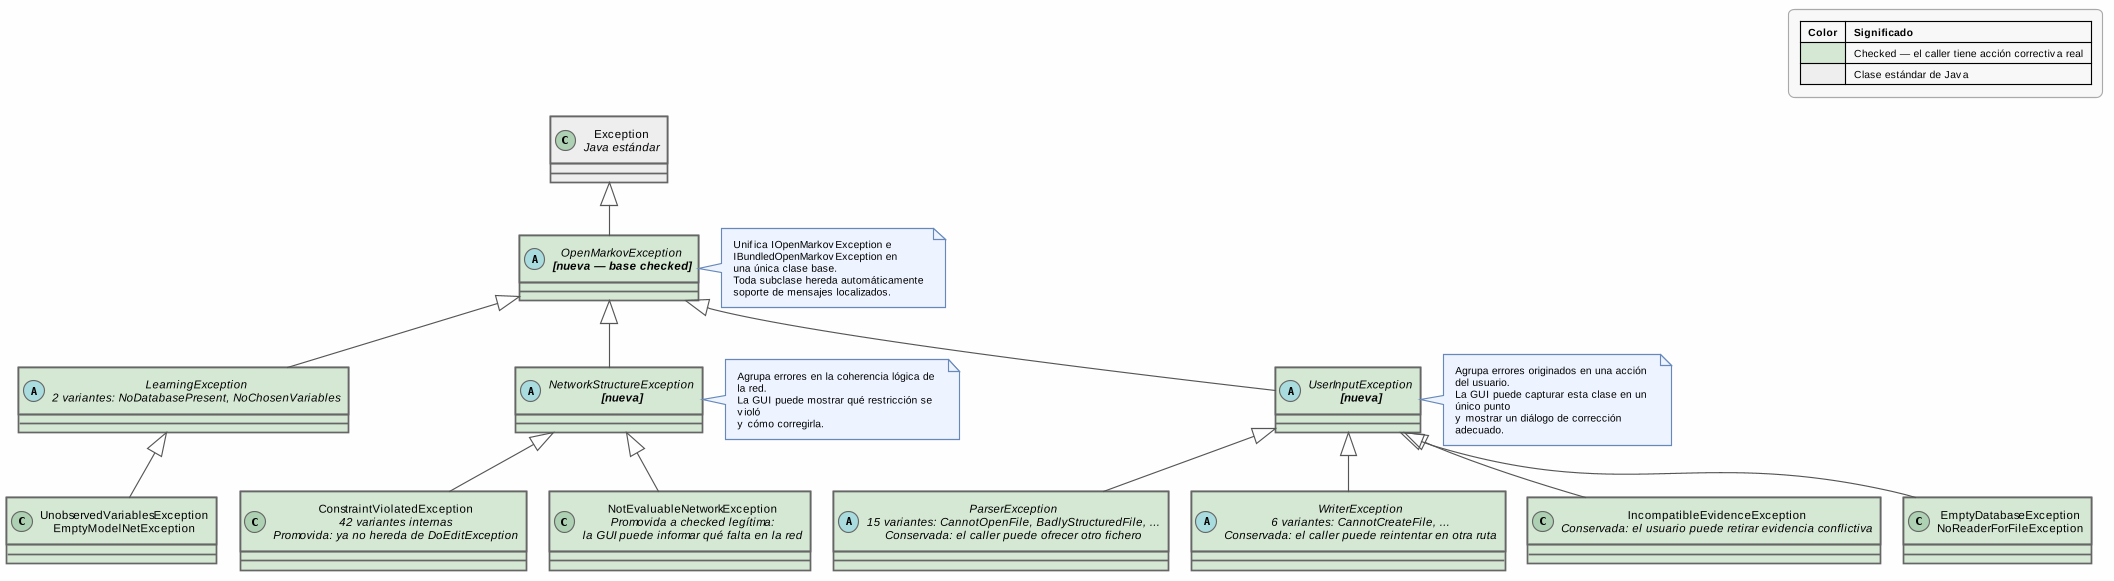
\includegraphics[width=\textwidth,keepaspectratio]{exception-hierarchy-proposed-checked}
    \caption{Jerarquía propuesta (parte~1): rama de excepciones \textit{checked} bajo
             \texttt{OpenMarkovException}. Fuente: \texttt{exception-hierarchy-proposed-checked.puml}.}
    \label{fig:jerarquia-propuesta-checked}
\end{figure}

\begin{figure}[htbp]
    \centering
    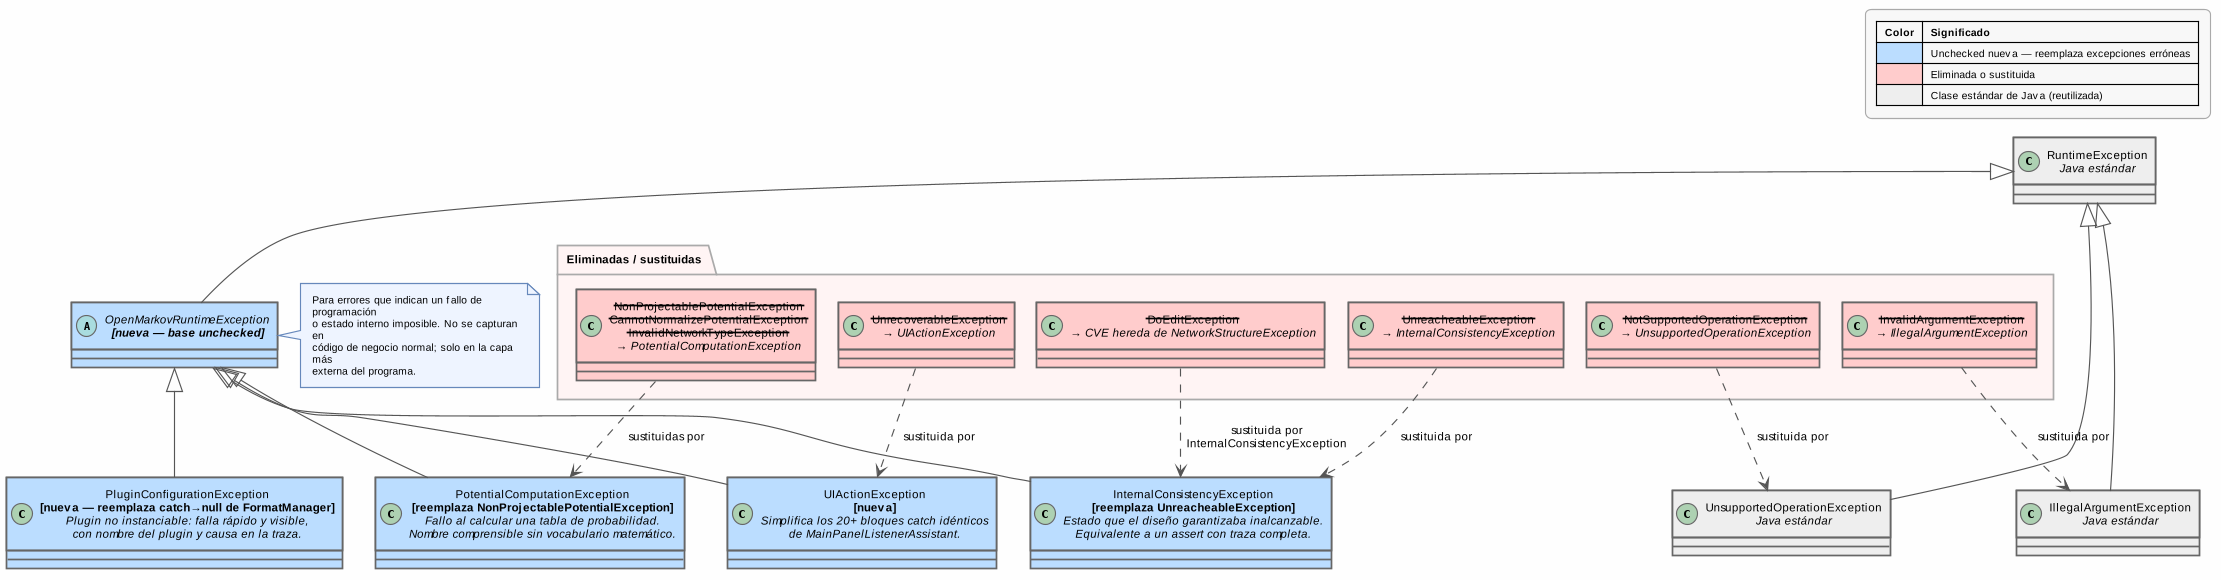
\includegraphics[width=\textwidth,keepaspectratio]{exception-hierarchy-proposed-unchecked}
    \caption{Jerarquía propuesta (parte~2): rama de excepciones \textit{unchecked} bajo
             \texttt{OpenMarkovRuntimeException}, con las clases eliminadas o sustituidas.
             Fuente: \texttt{exception-hierarchy-proposed-unchecked.puml}.}
    \label{fig:jerarquia-propuesta-unchecked}
\end{figure}

\subsubsection{Qué aporta la nueva jerarquía}

La reorganización propuesta introduce dos ramas claras, separadas por criterio de uso, no de módulo:

\paragraph{\texttt{OpenMarkovException} (base de las excepciones comprobadas).}
Unifica las actuales interfaces \texttt{IOpenMarkovException} e \texttt{IBundledOpenMarkovException}
en una única clase base concreta. Esto elimina la dualidad actual (dos interfaces, implementadas
de forma inconsistente según la excepción) y garantiza que cualquier excepción comprobada de
OpenMarkov tenga automáticamente soporte para mensajes localizados en el idioma del usuario.

\paragraph{\texttt{UserInputException}.}
Agrupa todos los errores que tienen su origen directo en una acción del usuario: abrir un fichero
con formato incorrecto, intentar escribir en una ruta sin permisos, introducir evidencia
contradictoria. La GUI puede capturar \texttt{UserInputException} en un único punto y mostrar
un diálogo de corrección adecuado, sin necesidad de conocer si el error vino de un
\texttt{ParserException} o de un \texttt{WriterException}.

\paragraph{\texttt{NetworkStructureException}.}
Agrupa los errores relacionados con la consistencia lógica de la red probabilística:
restricciones violadas, tipo de red inválido para la operación solicitada, red que no puede
evaluarse en el estado actual. Estos errores son recuperables: la GUI puede mostrar exactamente
qué restricción se violó y guiar al usuario a corregirla. Al separarlos en una rama propia, el
código de la GUI puede distinguir \guillemotleft el usuario ha hecho algo que viola una regla de la red\guillemotright 
de \guillemotleft ha ocurrido un error interno inesperado\guillemotright .

\paragraph{\texttt{OpenMarkovRuntimeException} (base de las excepciones no comprobadas).}
Todos los errores que representan fallos de programación o estados imposibles según el diseño
se unifican bajo esta base. Nadie en el código de negocio normal captura esta excepción; solo
la capa más externa del programa la captura para registrar el error y mostrar un mensaje
genérico al usuario.

\paragraph{\texttt{InternalConsistencyException}.}
Reemplaza a \texttt{UnreacheableException} (con el typo corregido). Se lanza cuando el
programa alcanza un punto de código que el diseño garantizaba inalcanzable: por ejemplo, un
valor de un \texttt{enum} que no está cubierto por un \texttt{switch}. En lugar de fallar con
una excepción poco descriptiva, esta excepción incluye suficiente contexto para que un
desarrollador identifique inmediatamente qué suposición de diseño se ha violado.

\paragraph{\texttt{PotentialComputationException}.}
Reemplaza a \texttt{NonProjectablePotentialException}. El nuevo nombre es más descriptivo para
cualquier desarrollador que no conozca el término matemático \guillemotleft potencial proyectable\guillemotright . Siendo
\textit{unchecked}, elimina las decenas de declaraciones \texttt{throws} en cascada que
actualmente impregnan el módulo de inferencia.

\paragraph{\texttt{PluginConfigurationException}.}
Excepción nueva que reemplaza el antipatrón \texttt{catch → null} de \texttt{FormatManager}.
Al ser \textit{unchecked}, se propaga automáticamente hasta la capa de gestión de errores de
la aplicación, donde se registra con el contexto completo (nombre del plugin, causa original).

\paragraph{\texttt{UIActionException}.}
Excepción nueva. Permite reemplazar los más
de veinte bloques \texttt{catch} idénticos en \texttt{MainPanelListenerAssistant} por un único
wrapper funcional:

\begin{lstlisting}[caption={Simplificación de los bloques \texttt{catch} de la GUI con \texttt{UIActionException}},label={lst:ui-action}]
// ANTES — repetido 20+ veces
case GO_TO_NEXT_EVIDENCE_CASE -> {
    try {
        evidenceCasesNavigationOption("GO_TO_NEXT_EVIDENCE_CASE");
    } catch (NotEvaluableNetworkException
           | NonProjectablePotentialException
           | NotEnoughtMemoryException
           | IncompatibleEvidenceException
           | CannotNormalizePotentialException
           | ThereIsNoNextEvidenceCaseException
           | ThereIsNoPreviousEvidenceCaseException
           | ConstraintViolatedException ex) {
        throw new UnrecoverableException(ex);
    }
}

// DESPUÉS — un único wrapper funcional
case GO_TO_NEXT_EVIDENCE_CASE ->
    executeUIAction(() -> evidenceCasesNavigationOption("GO_TO_NEXT_EVIDENCE_CASE"));

// Implementación del wrapper
void executeUIAction(UIAction action) {
    try {
        action.execute();
    } catch (OpenMarkovException ex) {
        throw new UIActionException(ex);
    }
}
\end{lstlisting}

\subsection{Propuesta F — Corrección de typos y conflictos de nombres}

\textbf{Impacto: bajo. Riesgo: muy bajo.}

Renombrar las ocho clases con errores ortográficos. Al ser en su mayoría clases internas o
clases con pocas referencias externas, el impacto es limitado y puede hacerse con herramientas
de refactorización automática del IDE (que actualizan todas las referencias en un único paso).

Resolver los conflictos de sombra (\texttt{WriterException\jdot NonProjectablePotentialException},
\texttt{PGMXParserException\jdot EvidenceIsIncompatibleWithOther}) eliminando las clases internas
duplicadas y usando directamente las clases raíz correspondientes.

\subsection{Propuesta G — Ocultar excepciones de infraestructura en las APIs de I/O}

\textbf{Impacto: medio. Riesgo: bajo.}

Los métodos que hoy declaran \texttt{throws SAXException, IOException} deben envolver esas
excepciones en tipos propios del dominio:

\begin{lstlisting}[caption={API limpia — sin exposición de detalles de implementación},label={lst:api-clean}]
// ANTES — acopla al llamador con SAX y con java.io
public ProbNetReader getProbNetReader(URL url)
    throws SAXException, IOException,
           NoReaderForFileException, ParserException;

// DESPUÉS — solo tipos del dominio de OpenMarkov
public ProbNetReader getProbNetReader(URL url)
    throws NoReaderForFileException, ParserException;
// SAXException e IOException quedan capturadas internamente
// y envueltas en ParserException como causa raíz
\end{lstlisting}

\subsection{Propuesta H — Corrección de la pérdida de traza en \texttt{DoEditException}}

\textbf{Impacto: bajo. Riesgo: muy bajo.}

En \texttt{Node.java} (línea 807), sustituir:

\begin{lstlisting}[caption={Corrección de la causa raíz perdida en \texttt{Node.java}},label={lst:node-fix}]
// ANTES — pierde el stack trace original
throw new DoEditException.CannotDoEditException(e.getMessage());

// DESPUÉS — preserva la causa completa
throw new DoEditException.CannotDoEditException(e);
\end{lstlisting}

Esta corrección tiene impacto únicamente en la calidad del diagnóstico: el comportamiento
observable para el usuario no cambia, pero los desarrolladores dispondrán de la traza de pila
completa cuando investiguen un fallo.

\subsection{Propuesta I — Eliminación del re-lanzamiento vacío en \texttt{setNetworkType()}}

\textbf{Impacto: bajo. Riesgo: muy bajo.}

En \texttt{ProbNet.java} (líneas 362--368), eliminar el bloque \texttt{try/catch} sin
tratamiento y dejar que la excepción se propague directamente:

\begin{lstlisting}[caption={Eliminación del bloque \texttt{try/catch} vacío en \texttt{ProbNet.java}},label={lst:probnet-fix}]
// ANTES — bloque vacío sin valor añadido
public void setNetworkType(NetworkType networkType)
        throws ConstraintViolatedException {
    try {
        // lógica de cambio de tipo
    } catch (ConstraintViolatedException e) {
        throw e;  // no hace nada
    }
}

// DESPUÉS — propagación directa, mismo comportamiento
public void setNetworkType(NetworkType networkType)
        throws ConstraintViolatedException {
    // lógica de cambio de tipo
    // la excepción se propaga sola si ocurre
}
\end{lstlisting}

\subsection{Propuesta J — Revisión de la lógica de navegación de evidencia}

\textbf{Impacto: medio. Riesgo: bajo.}

Las excepciones \texttt{ThereIsNoNext\-Evidence\-Case\-Exception} y
\texttt{ThereIsNoPrevious\-Evidence\-Case\-Exception} revelan un problema de diseño en la
navegación de evidencias. La corrección tiene dos niveles:

\begin{enumerate}
    \item \textbf{Corrección inmediata}: convertir estas excepciones a \textit{unchecked}
          para eliminar los bloques \texttt{catch} redundantes. Ambas se convierten en subclases
          de \texttt{OpenMarkovRuntimeException}, señalando que representan un uso incorrecto del
          API (intentar navegar más allá del límite sin verificar primero).

    \item \textbf{Corrección de diseño}: consultar el estado de la lista de evidencias
          \emph{antes} de habilitar o deshabilitar los botones de navegación. La GUI debe
          escuchar los cambios en la lista de evidencias y actualizar el estado de los botones
          en consecuencia, de forma que el usuario nunca pueda pulsar \guillemotleft siguiente\guillemotright  cuando ya
          está en el último caso.
\end{enumerate}

\begin{lstlisting}[caption={Enfoque preventivo para los botones de navegación de evidencia},label={lst:evidence-fix}]
// En EvidenceManager o equivalente
void onEvidenceCaseListChanged(List<EvidenceCase> cases, int currentIndex) {
    buttonNext.setEnabled(currentIndex < cases.size() - 1);
    buttonPrevious.setEnabled(currentIndex > 0);
    // Las excepciones de "no hay siguiente/anterior" nunca llegarán a lanzarse
}
\end{lstlisting}

\newpage

% ─────────────────────────────────────────────────────────────────────────────
\section{Plan de migración}
% ─────────────────────────────────────────────────────────────────────────────

La siguiente tabla organiza todas las propuestas en fases de riesgo creciente, de forma que
cada fase mejora la situación sin depender de que las fases posteriores estén completas:

\begin{longtable}{p{0.4cm}p{8.5cm}p{2.5cm}p{2cm}}
    \toprule
    \textbf{\#} & \textbf{Cambio} & \textbf{Propuesta} & \textbf{Riesgo} \\
    \midrule
    \multicolumn{4}{l}{\textbf{Fase 1 — Inmediata (sin impacto en lógica de negocio)}} \\
    \midrule
    1 & Corregir 8 typos en nombres de clase        & F & Muy bajo \\
    2 & Eliminar clases internas con nombre duplicado & F & Muy bajo \\
    3 & Corregir \texttt{catch → null} en \texttt{FormatManager} & D & Muy bajo \\
    4 & Preservar causa raíz en \texttt{Node.java} & H & Muy bajo \\
    5 & Eliminar bloque \texttt{try/catch} vacío en \texttt{setNetworkType()} & I & Muy bajo \\
    \midrule
    \multicolumn{4}{l}{\textbf{Fase 2 — Corto plazo (requiere actualizar los callers)}} \\
    \midrule
    6  & Convertir a \textit{unchecked}: \texttt{InvalidArgumentException} → \texttt{IllegalArgumentException} & A & Bajo \\
    7  & Convertir a \textit{unchecked}: \texttt{NotSupportedOperationException} → \texttt{Unsupported\-OperationException} & A & Bajo \\
    8  & Convertir a \textit{unchecked}: \texttt{NoSelectedNodeException}, \texttt{WrongClass\-Exception}, \texttt{UnexpectedMenu\-ActionException} & A & Bajo \\
    9  & Convertir a \textit{unchecked}: \texttt{ThereIsNoNext/Previous\-EvidenceCaseException} & J & Bajo \\
    10 & Convertir a \textit{unchecked}: \texttt{InvalidNetwork\-TypeException}, \texttt{CannotNormalize\-PotentialException}, \texttt{Unexpected\-InferenceException} & A & Medio \\
    11 & Ocultar \texttt{SAXException}/\texttt{IOException} en APIs de I/O & G & Bajo \\
    \midrule
    \multicolumn{4}{l}{\textbf{Fase 3 — Medio plazo (eliminar throws genéricos)}} \\
    \midrule
    12 & Especificar \texttt{throws Exception} en \texttt{LearningAlgorithm} & C & Bajo \\
    13 & Convertir a \textit{unchecked}: \texttt{NonProjectablePotentialException} → \texttt{PotentialComputationException} & A+E & Medio \\
    14 & Crear \texttt{UIActionException} y consolidar bloques \texttt{catch} de la GUI & J & Medio \\
    15 & Revisar lógica de botones de navegación de evidencia (enfoque preventivo) & J & Bajo \\
    \midrule
    \multicolumn{4}{l}{\textbf{Fase 4 — Largo plazo (reestructuración jerárquica completa)}} \\
    \midrule
    16 & Introducir \texttt{OpenMarkovException} como base \textit{checked} unificada & E & Alto \\
    17 & Introducir \texttt{UserInputException} y \texttt{NetworkStructureException} & E & Alto \\
    18 & Introducir \texttt{OpenMarkovRuntimeException} e \texttt{InternalConsistencyException} & E & Alto \\
    19 & Migrar \texttt{DoEditException}: \texttt{ConstraintViolatedException} hereda de \texttt{NetworkStructureException} directamente & E & Alto \\
    \bottomrule
\end{longtable}

Las fases 1 a 3 son completamente independientes entre sí y mejoran la situación de forma
incremental. La fase 4 es una refactorización estructural mayor que conviene abordar cuando
las capas de aplicación estén estabilizadas y exista cobertura de tests suficiente para
verificar que el comportamiento observable no ha cambiado.

\end{document}
